\newpage

\subsubsection{UCA 5 - Visualizzazione dello storico accessi presso un'organizzazione}
\begin{figure}[h]
	\centering	
	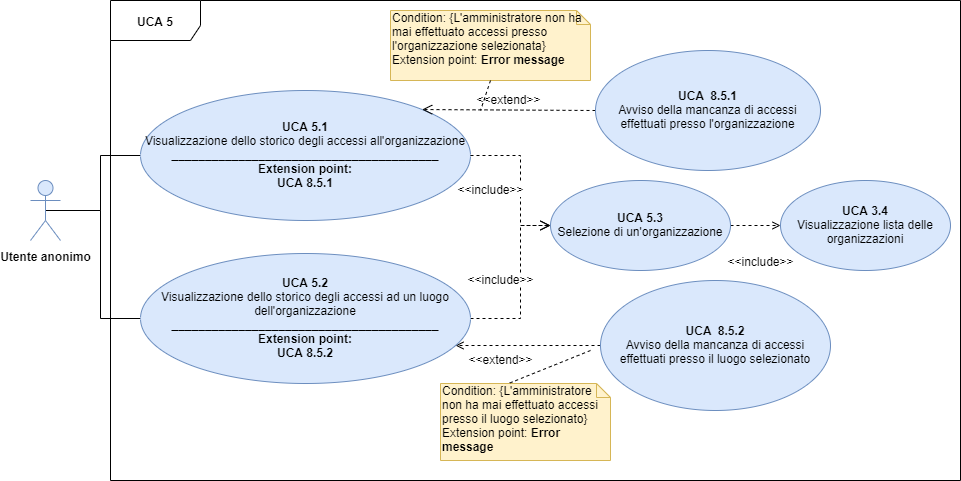
\includegraphics[scale=0.5]{sezioni/UseCase/Immagini/UCA5.png}
	\caption{UCA 5 - Visualizzazione dello storico accessi presso un'organizzazione}
\end{figure}

\begin{itemize}
    \item \textbf{Attori primari:} Utente anonimo, Utente riconosciuto
    \item \textbf{Precondizione:} L'utente ha precedentemente scaricato la lista delle organizzazioni.
    \item \textbf{Postcondizione:} L'utente visualizza la lista degli accessi effettuati presso l'organizzazione.
    \item \textbf{Scenario principale:} L'utente può visualizzare la lista dei propri accessi (con nome dell'organizzazione, timestamp di ingresso, di uscita, e tempo di permanenza) presso un'organizzazione. Se si trova all'interno dell'organizzazione stessa, viene visualizzato il tempo passato al suo interno dall'ultimo ingresso effettuato.
    \item \textbf{Scenario alternativo:} L'utente non è mai entrato nell'area selezionata, pertanto verra visualizzato un avviso informativo [UCA 7.5.1].
    \item \textbf{Flusso di eventi:}
    \begin{enumerate}
        \item L'utente visualizza la lista delle organizzazioni [UCA 3.4];
        \item L'utente seleziona dalla lista l'organizzazione interessata;
    \end{enumerate}
    \item \textbf{Inclusioni:}
    \begin{itemize}
        \item UCA 3.4 - Visualizzazione lista delle organizzazioni;
    \end{itemize}
    \begin{itemize}
        \item UCA 7.5.1 - Avviso della mancanza di accessi effettuati presso l'organizzazione selezionata.
    \end{itemize}
\end{itemize}


\subsubsection{UCA 5.1 - Visualizzazione dello storico degli accessi ad un luogo dell'organizzazione}
\begin{itemize}
    \item \textbf{Attori primari:} Utente anonimo, Utente riconosciuto
    \item \textbf{Precondizione:} L'utente sta visualizzando lo storico accessi di un'organizzazione [UCA 5] e l'organizzazione in questione deve avere almeno un luogo registrato.
    \item \textbf{Postcondizione:} L'utente visualizza lo storico degli accessi al luogo desiderato.
    \item \textbf{Scenario principale:} L'utente selezionerà il luogo desiderato per vedere il relativo storico degli accessi. Se l'utente dovesse trovarsi all'interno del luogo stesso, viene visualizzato il tempo passato al suo interno dall'ultimo ingresso effettuato.
    \item \textbf{Scenario alternativo:} L'utente non è mai entrato nel luogo selezionato, pertanto verra mostrato un avviso informativo [UCA 7.5.2].
    \item \textbf{Flusso di eventi:}
    \begin{enumerate}
        \item L'utente seleziona il luogo desiderato tra quelli offerti dall'organizzazione.
    \end{enumerate}
    \item \textbf{Estensioni:}
    \begin{itemize}
        \item UCA 7.5.2 - Avviso della mancanza di accessi effettuati presso il luogo selezionato.
    \end{itemize}
\end{itemize}

\subsubsection{UCA 5.1.1 - Ordinamento per data decrescente della lista degli accessi presso un'organizzazione}
\begin{itemize}
    \item \textbf{Attori primari:} Utente anonimo, Utente riconosciuto
    \item \textbf{Precondizione:} L'utente sta visualizzando lo storico accessi di un'organizzazione [UCA 5].
    \item \textbf{Flusso di eventi:}
    \begin{enumerate}
        \item L'utente seleziona la funzionalità per riordinare lo storico di accessi dell'organizzazione per data in ordine decrescente.
    \end{enumerate}
    \item \textbf{Postcondizione:} L'utente ottiene la lista di accessi iniziale riordinata per data in ordine decrescente.
\end{itemize}

\subsubsection{UCA 5.1.2 - Ordinamento per data crescente della lista degli accessi presso un'organizzazione}
\begin{itemize}
    \item \textbf{Attori primari:} Utente anonimo, Utente riconosciuto
    \item \textbf{Precondizione:} L'utente sta visualizzando lo storico accessi di un'organizzazione [UCA 5].
    \item \textbf{Flusso di eventi:}
    \begin{enumerate}
        \item L'utente seleziona la funzionalità per riordinare lo storico di accessi dell'organizzazione per data in ordine crescente.
    \end{enumerate}
    \item \textbf{Postcondizione:} L'utente ottiene la lista di accessi iniziale riordinata per data in ordine crescente.
\end{itemize}

\subsubsection{UCA 5.1.3 - Ricerca degli accessi presso un'organizzazione in un giorno specifico}
\begin{itemize}
    \item \textbf{Attori primari:} Utente anonimo, Utente riconosciuto
    \item \textbf{Precondizione:} L'utente sta visualizzando lo storico accessi di un'organizzazione [UCA 5].
    \item \textbf{Flusso di eventi:}
    \begin{enumerate}
        \item L'utente seleziona la funzionalità per visualizzare solo gli acessi avvenuti in un giorno specifico presso l'organizzazione;
        \item L'utente seleziona il giorno desiderato.
    \end{enumerate}
    \item \textbf{Postcondizione:} L'utente ottiene la lista di accessi effettuati nel giorno selezionato.
\end{itemize}

\subsubsection{UCA 5.2.1 - Ordinamento per data decrescente della lista degli accessi presso un luogo di un'organizzazione}
\begin{itemize}
    \item \textbf{Attori primari:} Utente anonimo, Utente riconosciuto
    \item \textbf{Precondizione:} L'utente sta visualizzando lo storico accessi di un luogo [UCA 5.1].
    \item \textbf{Flusso di eventi:}
    \begin{enumerate}
        \item L'utente seleziona la funzionalità per riordinare lo storico di accessi del luogo per data in ordine decrescente.
    \end{enumerate}
    \item \textbf{Postcondizione:} L'utente ottiene la lista di accessi iniziale riordinata per data in ordine decrescente.
\end{itemize}

\subsubsection{UCA 5.2.2 - Ordinamento per data crescente della lista degli accessi presso un luogo di un'organizzazione}
\begin{itemize}
    \item \textbf{Attori primari:} Utente anonimo, Utente riconosciuto
    \item \textbf{Precondizione:} L'utente sta visualizzando lo storico accessi di un luogo [UCA 5.1].
    \item \textbf{Flusso di eventi:}
    \begin{enumerate}
        \item L'utente seleziona la funzionalità per riordinare lo storico di accessi del luogo per data in ordine crescente.
    \end{enumerate}
    \item \textbf{Postcondizione:} L'utente ottiene la lista di accessi iniziale riordinata per data in ordine crescente.
\end{itemize}

\subsubsection{UCA 5.2.3 - Ricerca degli accessi presso un luogo di un'organizzazione in un giorno specifico}
\begin{itemize}
    \item \textbf{Attori primari:} Utente anonimo, Utente riconosciuto
    \item \textbf{Precondizione:} L'utente sta visualizzando lo storico accessi di un luogo [UCA 5.1].
    \item \textbf{Flusso di eventi:}
    \begin{enumerate}
        \item L'utente seleziona la funzionalità per visualizzare solo gli acessi avvenuti in un giorno specifico presso il luogo in questione dell'organizzazione;
        \item L'utente seleziona il giorno desiderato.
    \end{enumerate}
    \item \textbf{Postcondizione:} L'utente ottiene la lista di accessi effettuati presso il luogo in questione nel giorno selezionato.
\end{itemize}